% \documentclass[8pt,xcolor=pdftex,table,handout]{beamer}

\documentclass[8pt,xcolor=pdftex,table]{beamer}
\include{preambule_beamer}

\usepackage{listings}

% \usepackage{amsmath}
% \usepackage{unicode-math}
% \setmathfont{Fira Math}


% \usepackage{animate}

% ------------------------------------------- %

\graphicspath{{Figures/} {Figures/Logos/} {../Figures/}}
% \graphicspath{{../Figures/} {../Figures/Logos/}}

\title[]{\vspace{22mm}Formation \alert{Ingénieur Machine Learning}\\\vspace{6mm}Projet:\\\alert{Classez des images à l'aide d'algorithmes de Deep Learning}}
\date[]{14 Juillet 2023\\\vspace{18mm}\\\tit{thomas.durandtexte@protonmail.com}}


\titlegraphic{\hfill
\def\arraystretch{.1}%  1 is the default, change whatever you need
	\begin{tabular}{ >{\centering}m{7mm} m{39mm} }
		
\includegraphics[height=7mm]{Logo_OpenClassrooms.png }
		&
		\Large{\textbf{OPENCLASSROOMS}}
	\end{tabular}
}

% \definecolor{clrData}{rgb}{0.9,0.5,0}

\tikzstyle{box_style00}=[draw, rounded corners,anchor=center,text centered,text=white]
% \tikzstyle{diagram0}=[box_style00, text width=22mm, minimum height=12mm]
% \tikzstyle{dataset}=[box_style00,diagram0, fill=blue]
% \tikzstyle{filtrage}=[box_style00,diagram0, fill=red!80]
% \tikzstyle{doublons}=[box_style00,diagram0, fill=magenta!80]
% \tikzstyle{datavoisins}=[box_style00,diagram0, fill=cyan!80]
% \tikzstyle{outliers}=[box_style00,diagram0, fill=magenta!80]

% \includeonlyframes{CCL,Merci}



\begin{document}
% ------------------------------------------- %

\begin{frame}
	\titlepage{}
\end{frame}


\section{CONTEXTE}


\begin{frame}[t, label=contexte]
	\vspace{0mm}
	\centering
	\vfill
	\begin{tikzpicture}
		\linespread{1}% <--- locally defined vertical line spacing in nodes
		\drawBorder
		\nodePageNumber

		\onlystyle<2->{removed}{myShaded}
		\node[box_style00, text width = 40mm, removed] at (0.5\txw,80mm)
			{Aide pour une association de protection des animaux} ;

		\visible<2->{
		\node[box_style00] at (0.5\txw, 60mm) (I)
			{Images de chiens \alert{à trier}} ;
		}
		\visible<3->{
			\node[box_style00] at (0.5\txw, 40mm) (DL)
				{Modèle \alert{Deep Learning}} ;
			\draw[myarrow] (I) -- (DL) ;
		}

		\visible<4->{
			\node[box_style00] at (0.5\txw, 20mm) (I2)
				{Images de chiens \alert{triées}} ;
			\draw[myarrow] (DL) -- (I2) ;
		}
	\end{tikzpicture}
	\vfill
\end{frame}


\subsection{Base de données}
\begin{frame}[t, label=BaseDonnees]
	\vspace{0mm}
	\centering
	\vfill
	\begin{tikzpicture}
		\linespread{1}% <--- locally defined vertical line spacing in nodes
		\drawBorder
		% \draw[clrBorders] (1.25mm,1.25mm) rectangle (\txw-1.25mm,\txh-1.25mm) ;
		% \draw[clrBorders] (0,0) rectangle (\txw,\txh) ;
		\nodePageNumber

		\onlystyle<2->{shd1}{myShaded}
		\onlystyle<4->{shd2}{myShaded}

		\visible<1->{
			\node[box_style00, shd1] (Dataset) at (\midX,80mm) {Stanford Dogs Dataset} ;
		}

		\begin{scope}[yshift=70mm]
			\visible<2->{
				\node[box_style00, shd2] (Images) at (0.3\txw,0) {20580 images} ;
				\draw[myarrow, shd2] (Dataset) |- (Images) ;
			}

			\visible<3->{
				\node[box_style00, shd2] (Classes) at (0.7\txw,0) {120 classes} ;
				\draw[myarrow, shd2] (Dataset) |- (Classes) ;
			}
		\end{scope}

		\node at (\midX,38mm) {
			\includegraphics<4>[width=80mm]{explore/n_images_per_classe-0.pdf}%
			\includegraphics<5->[width=80mm]{explore/n_images_per_classe.pdf}
		} ;

		\node<6> at (\midX, 10mm) {\alert{4244 images} utilisées} ;
	\end{tikzpicture}
	\vfill
\end{frame}


\subsection{Protocole}
\begin{frame}[t, label=protocol]
	\vspace{0mm}
	\centering
	\vfill
	\begin{tikzpicture}
		\linespread{1}% <--- locally defined vertical line spacing in nodes
		\drawBorder
		\nodePageNumber


		\onlystyle<2->{shd1}{myShaded}
		\onlystyle<3->{shd2}{myShaded}
		\onlystyle<4->{shd3}{myShaded}
		\onlystyle<6->{shd4}{myShaded}
		\onlystyle<7->{shd5}{myShaded}
		\onlystyle<8->{shd6}{myShaded}
		\onlystyle<9->{shd7}{myShaded}

		\begin{scope}[xshift=35mm]
			\node[box_style00,shd1] (Decouverte) at (0mm,80mm) {Découverte des modèles existants} ;

			\visible<2->{
				\node[box_style00, text width=20mm, shd2] (FromScratch) at (-15mm, 60mm) {Création d'un modèle \alert<-4>{from scratch}} ;
				\draw[myarrow,shd2] (Decouverte) -- ++(0,-9mm) -| (FromScratch) ;
			}
			\visible<3->{
				\node[box_style00,shd4, text width=20mm] (TrainTest) at (-15mm, 40mm) {Entrainement et Analyse} ;
				\draw[myarrow,shd3] (FromScratch) -- ++(0,-9mm) -| (TrainTest) ;
			}

			\visible<4->{
				\node[box_style00,shd4, text width=20mm] (Update) at (15mm, 40mm) {Modifications} ;
				\draw[myarrow,shd4] (TrainTest) -- (Update) ;
			}

			\visible<5->{
				\draw[myarrow,shd4] (Update) -- ++(0, 10mm) -| (TrainTest) ;
				\node[shd4] at (0,46mm) {\textit{loop}} ;
			}

			\visible<6->{
				\node[box_style00,shd5, text width=20mm] (ccls) at (-15mm,20mm) {Conclusions} ;
				\draw[myarrow,shd4] (TrainTest) -- (ccls) ;
			}
		\end{scope}


		\begin{scope}[xshift=80mm]
			\node<7->[box_style00, shd6, text width=20mm] (PreTrained) at (0,60mm) {Chargement d'un modèle \alert<7>{pré-entrainé}} ;
			\draw<7->[myarrow, shd6] (Decouverte) -- ++ (0, -9mm) -| (PreTrained);

			\node<8->[box_style00, shd7, text width=20mm] (Train2) at (0, 40mm) {Entrainement} ;
			\draw<8->[myarrow, shd7] (PreTrained) -- ++ (0, -9mm) -| (Train2);

			\node<9->[box_style00, text width=20mm] (ccls2) at (0, 20mm) {Conclusions} ;
			\draw<9->[myarrow] (Train2) -- (ccls2);
		\end{scope}


		% \visible<7->{
		% 	\node[text width=40mm, text centered] at (83mm,20mm) {Essais de\\différents classifieurs} ;
		% }
	\end{tikzpicture}
	\vfill
\end{frame}


\section{EXPLORATION DES DONNÉES}

\begin{frame}[t, label=classExamples]
	\vspace{0mm}
	\centering
	\vfill
	\begin{tikzpicture}
		\linespread{1}% <--- locally defined vertical line spacing in nodes
		\drawBorder
		\nodePageNumber

		\onlystyle<2->{shd1}{myShaded}
		\node[shd1] at (\midX,80mm) {Exemple d'images} ;

		\node at (\midX,60mm) {
			\includegraphics<2-3>[width=80mm]{explore/class_examples/Afghan_hound.pdf}%
			\includegraphics<4->[width=80mm]{explore/class_examples/Australian_terrier.pdf}
			} ;
		\node at (\midX,25mm) {
			\includegraphics<3-4>[width=80mm]{explore/class_examples/Airedale.pdf}%
			\includegraphics<5->[width=80mm]{explore/class_examples/Basenji.pdf}
			} ;

		\node<6> at (\midX,\midY-3mm) {Les \alert{images couleurs} sont utilisées} ;

	\end{tikzpicture}
	\vfill
\end{frame}


\begin{frame}[t, label=imgShapes]
	\vspace{0mm}
	\centering
	\vfill
	\begin{tikzpicture}
		\linespread{1}% <--- locally defined vertical line spacing in nodes
		\drawBorder
		\nodePageNumber

		% \onlystyle<2->{shd1}{myShaded}
		% \node[shd1] at (\midX,85	mm) {Décompte des dimensions des images} ;

		\node at (\midX,\midY) {
			\includegraphics<1>[width=80mm]{explore/count_shapes-0.pdf}%
			\includegraphics<2>[width=80mm]{explore/count_shapes.pdf}
			} ;
		\node<2> at (45mm,72mm) {(maximum)} ;

	\end{tikzpicture}
	\vfill
\end{frame}

\subsection{Pre-processing}
\begin{frame}[t, label=preprocessing]
	\vspace{0mm}
	\centering
	\vfill
	\begin{tikzpicture}
		\linespread{1}% <--- locally defined vertical line spacing in nodes
		\drawBorder
		\nodePageNumber

		\onlystyle<2->{shd1}{myShaded}
		\onlystyle<3->{shd2}{myShaded}
		\onlystyle<4->{shd3}{myShaded}
		\onlystyle<5->{shd4}{myShaded}
		\node[shd1] at (\midX,80mm) {Pre-processing} ;

		\node<2-5>[box_style00, shd2, text width=30mm] (Filtre) at (\midX, 65mm) {Filtrage gaussien\\ $\sigma \propto$ max(H, W) / 224} ;

		\node<3-5>[box_style00, shd3, text width=30mm] (Resize) at (\midX, 50mm) {Redimensionnement:\\ max(H, W) $\rightarrow$ 224} ;
		\draw<3-5>[myarrow, shd3] (Filtre) -- (Resize) ;

		\node<4-5>[box_style00, shd4, text width=30mm] (Zeropad) at (\midX, 35mm) {Zeros padding:\\ 224 $\times$ 224} ;
		\draw<4-5>[myarrow, shd4] (Resize) -- (Zeropad) ;

		\node<5>[box_style00, text width=30mm] (Normalize) at (\midX, 20mm) {Normalisation} ;
		\draw<5>[myarrow] (Zeropad) -- (Normalize) ;


		\node<6-> at (\midX-23mm,65mm) {image brute} ;
		\node<6-> at (\midX-23mm,\midY) {
\includegraphics[width=45mm]{explore/test_process_raw.jpg}} ;
		\node<7-> at (\midX+23mm,\midY) {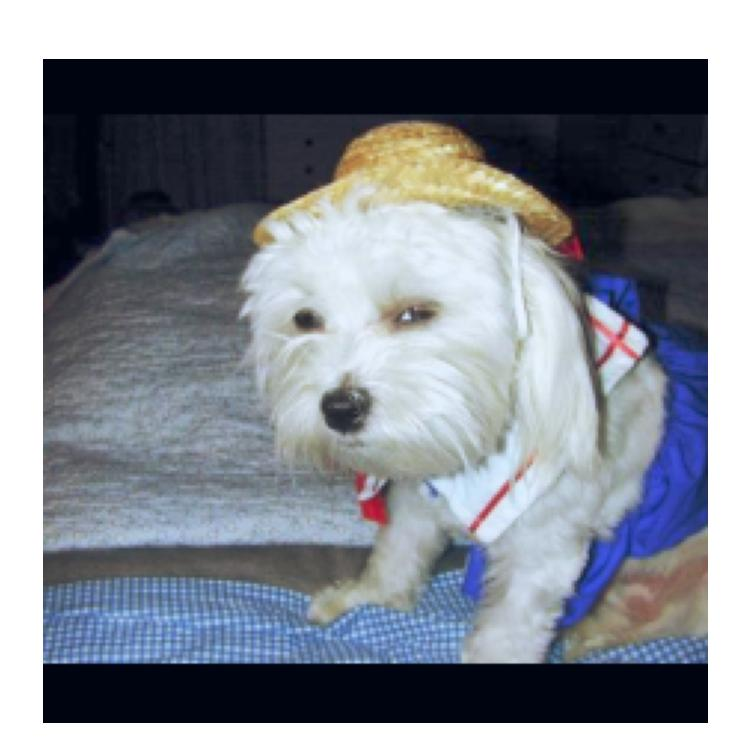
\includegraphics[width=45mm]{explore/test_process.jpg}} ;
		\node<7->[black] at (\midX+23mm,66.5mm) {image traitée} ;
		\node<8->[myOrng] at (\midX, 15mm) {Zero padding} ;
		\draw<8->[myarrow, myOrng] (\midX+0mm, 18mm) -- (\midX+13mm, 63mm) ;
		\draw<8->[myarrow, myOrng] (\midX+5mm, 18mm) -- (\midX+17mm, 27mm) ;
	\end{tikzpicture}
	\vfill
\end{frame}

\section{MODÉLISATIONS}

\subsection{Conventions}
\begin{frame}[t, label=ArchitectureType]
	\vspace{0mm}
	\centering
	\vfill
	\begin{tikzpicture}
		\linespread{1}% <--- locally defined vertical line spacing in nodes
		\drawBorder
		\nodePageNumber

		\onlystyle<2->{shd1}{myShaded}
		\onlystyle<3->{shd2}{myShaded}
		\onlystyle<4->{shd3}{myShaded}
		\onlystyle<5->{shd4}{myShaded}
		\onlystyle<6->{shd5}{myShaded}
		\onlystyle<7->{shd6}{myShaded}
		\node[shd1] at (\midX,80mm) {Architecture générale} ;

		\node<2->[box_style00, shd2] (image) at (\midX,\midY+20mm) {Image} ;
		\node<3->[box_style00, shd3, text width=20mm] (encodeur) at (\midX,\midY+5mm) {\alert<3,6>{Encodeur} :\\extraction de\\caractéristiques} ;
		\draw<3->[myarrow, shd3] (image) -- (encodeur) ;
		\node<4->[box_style00, shd4] (classifieur) at (\midX, \midY-10mm) {\alert<4,7>{Classifieur}} ;
		\draw<4->[myarrow, shd4] (encodeur) -- (classifieur) ;
		\node<5->[box_style00, shd5] (prediciton) at (\midX, \midY-25mm) {Prédiction} ;
		\draw<5->[myarrow, shd5] (classifieur) -- (prediciton);

		\begin{scope}[xshift=\midX+10mm, yshift=\midY]
			\draw<6->[shd6, decorate,decoration={brace,amplitude=7pt}] (4mm,12mm) -- (4mm,-2mm);
			\node<6->[shd6, text width=20mm, text centered] at (19mm,5mm) {couches\\convolutionnelles} ;

			\draw<7->[decorate,decoration={brace,amplitude=7pt}] (0,-5mm) -- (0,-15mm);
			\node<7->[text width=20mm, text centered] at (10mm,-10mm) {couches\\denses} ;
		\end{scope}


	\end{tikzpicture}
	\vfill
\end{frame}

\begin{frame}[t, label=couchesTypes]
	\vspace{0mm}
	\centering
	\vfill
	\begin{tikzpicture}
		\linespread{1}% <--- locally defined vertical line spacing in nodes
		\drawBorder
		\nodePageNumber

		\onlystyle<2->{shd1}{myShaded}
		\onlystyle<3->{shd2}{myShaded}
		\onlystyle<10->{shd3}{myShaded}
		\onlystyle<15->{shd4}{myShaded}
		\node[shd1] at (\midX,80mm) {Types de couches} ;

		\begin{scope}[xshift=\midX, yshift=\midY]
			\begin{scope}[yshift=20mm]
				\node<2->[shd2] at (0, 5mm) {couche convolutionnelle} ;
				\node<2->[conv]
					{Conv2d \highlight<3>{N:96}, \highlight<4>{(3$\times$3)}, \highlight<5>{s:1}, \highlight<6>{(S)}} ;
				\BatchNorm<7->{1} ;
				\Activation<8->{2} ;
				\begin{scope}[yshift=-10mm]
					\node<3> {\tit{nombre de filtres}} ;
					\node<4> {\tit{taille du noyau}} ;
					\node<5> {\tit{stride / pas entre deux filtres}} ;
					\node<6> {\tit{padding : "Valid" ou "Same"}} ;
					\node<7> {\tit{batch normalization}} ;
					\draw<7>[myarrow] (0, 1.2mm) -- ++ (0, 4.7mm) ;
					\node<8> {\tit{fonction d'activation}} ;
					\draw<8>[myarrow] (0, 1.4mm) -- ++ (0, 3.3mm) ;
				\end{scope}
			\end{scope}

			\begin{scope}[yshift=0mm]
				\node<9->[shd3] at (0, 5mm) {couche de pooling} ;
				\node<9->[pool] {\textcolor<10>{black}{Type} \textcolor<11>{black}{(3$\times$3)}, \textcolor<12>{black}{s:2}, \textcolor<13>{black}{(V)}} ;
				\begin{scope}[yshift=-10mm]
					\node<10> {\tit{(Global) Max / Average}} ;
					\node<11> {\tit{taille du noyau}} ;
					\node<12> {\tit{stride}} ;
					\node<13> {\tit{padding : "Valid" ou "Same"}} ;
				\end{scope}
			\end{scope}

			\begin{scope}[yshift=-20mm]
				\node<14->[shd4] at (0, 5mm) {couche de dense (linéaire)} ;
				\node<14->[dense] at (0,0)
					{Dense \highlight<15>{512} $\rightarrow$ \highlight<16>{128}} ;
				\BatchNorm<17->{1} ;
				\Activation<18->{2} ;
				\begin{scope}[yshift=-10mm]
					\node<15> {\tit{nombre de paramètres en entrée}} ;
					\node<16> {\tit{nombre de paramètres en sortie\phantom{\rule{1.07mm}{1mm}}}} ;
					\node<17> {\tit{batch normalization}} ;
					\draw<17>[myarrow] (0, 1.2mm) -- ++ (0, 4.7mm) ;
					\node<18> {\tit{fonction d'activation}} ;
					\draw<18>[myarrow] (0, 1.4mm) -- ++ (0, 3.3mm) ;
				\end{scope}
			\end{scope}

			% \begin{scope}[xshift=0, yshift=-3.3mm]
			% 	\fill[fill=cyan, rounded corners=0.5mm] (-17.5mm,-0.7mm) rectangle (17.5mm,0.7mm) ;
			% \end{scope}
		\end{scope}
	\end{tikzpicture}
	\vfill
\end{frame}

\begin{frame}[t, label=activationReLU]
	\vspace{0mm}
	\centering
	\vfill
	\begin{tikzpicture}
		\linespread{1}% <--- locally defined vertical line spacing in nodes
		\drawBorder
		\nodePageNumber

		\onlystyle<2->{shd1}{myShaded}
		\node[shd1] at (\midX,80mm) {Fonction d'activation} ;

		\node at (\midX,\midY) {
			\includegraphics<2->[width=80mm]{essais/activations_0.pdf}%
		} ;

		\node<3> at (\midX,15mm) {Ajout de non-linéarités} ;
	\end{tikzpicture}
	\vfill
\end{frame}

\subsection{Architecture initiale}
\begin{frame}[t, label=ModelInitial]
	\vspace{0mm}
	\centering
	\vfill
	\begin{tikzpicture}
		\linespread{1}% <--- locally defined vertical line spacing in nodes
		\drawBorder
		\nodePageNumber

		\onlystyle<2->{shd1}{myShaded}
		\onlystyle<3->{shd2}{myShaded}
		\onlystyle<9->{shd3}{myShaded}
		\node[shd1] at (\midX,80mm) {Architecture basée sur AlexNet} ;


		\begin{scope}[xshift=\midX-25mm]
			\begin{scope}[yshift=70mm]
				\node<2->[shd2] at (0, 5mm) {\tit{Encodeur}} ;
				\node<2->[conv]
					{Conv2d N:96, (7$\times$7), s:2, (V)} ;
				\BatchNorm<2->{1} ;
				\Activation<2->{2} ;
				\node (conv1) at (0, -3.8mm) {} ;
			\end{scope}

			\begin{scope}[yshift=57.5mm]
				\node<3->[pool] (pool1) {Max (5$\times$5), s:4, (V)} ;
				\draw<3->[myarrow] (conv1) -- (pool1) ;
			\end{scope}

			\begin{scope}[yshift=45mm]
				\node<4->[conv] (conv2Up)
				{Conv2d N:192, (5$\times$5), s:2, (V)} ;
				\BatchNorm<4->{1} ;
				\Activation<4->{2} ;
				\node (conv2) at (0, -3.8mm) {} ;
				\draw<4->[myarrow] (pool1) -- (conv2Up) ;
			\end{scope}

			\begin{scope}[yshift=32.5mm]
				\node<5->[pool] (pool2) {Max (3$\times$3), s:2, (V)} ;
				\draw<5->[myarrow] (conv2) -- (pool2) ;
			\end{scope}

			\begin{scope}[yshift=20mm]
				\node<6->[conv] (conv3Up)
				{Conv2d N:192, (3$\times$3), s:1, (V)} ;
				\BatchNorm<6->{1} ;
				\Activation<6->{2} ;
				\node (conv3) at (0, -3.8mm) {} ;
				\draw<6->[myarrow] (pool2) -- (conv3Up) ;
			\end{scope}

			\begin{scope}[yshift=7.5mm]
				\node<7->[pool] (pool3) {Global Max} ;
				\draw<7->[myarrow] (conv3) -- (pool3) ;
			\end{scope}
		\end{scope}

		\begin{scope}[xshift=\midX+25mm]
			\begin{scope}[yshift=60mm]
				\node<8->[shd3] at (0, 5mm) {\tit{Classifieur}} ;
				\node<8->[dense] (dense1Up)
					{Dense 192 $\rightarrow$ 128} ;
				\BatchNorm<8->{1} ;
				\Activation<8->{2} ;
				\node (dense1) at (0, -3.8mm) {} ;
				\draw<8->[myarrow] (pool3) -| (-25mm, -10mm) |- (dense1Up) ;
			\end{scope}

			\begin{scope}[yshift=40mm]
				\node<9->[dense] (dense2Up)
					{Dense 128 $\rightarrow$ 128} ;
				\BatchNorm<9->{1} ;
				\Activation<9->{2} ;
				\node (dense2) at (0, -3.8mm) {} ;
				\draw<9->[myarrow] (dense1) -- (dense2Up) ;
			\end{scope}

			\begin{scope}[yshift=20mm]
				\node<10->[dense] (dense3)
					{Dense 128 $\rightarrow$ N classes} ;
				\draw<10->[myarrow] (dense2) -- (dense3) ;
			\end{scope}

			\node<11>[clrFactiv] at (0, 72mm) {activation: \tbf{ReLU}} ;
		\end{scope}

	\end{tikzpicture}
	\vfill
\end{frame}

\subsection{Algorithme type Levenberg-Marquardt}
\begin{frame}[t, label=AlgoLM]
	\vspace{0mm}
	\centering
	\vfill
	\begin{tikzpicture}
		\linespread{1}% <--- locally defined vertical line spacing in nodes
		\drawBorder
		\nodePageNumber

		\onlystyle<2->{shd1}{myShaded}
		\onlystyle<3->{shd2}{myShaded}
		\onlystyle<4->{shd3}{myShaded}
		\onlystyle<6->{shd4}{myShaded}
		\onlystyle<8->{shd5}{myShaded}
		\node[shd1] at (\midX,80mm) {Algorithme type Levenberg-Marquardt} ;

		\begin{scope}[xshift=\midX, yshift=\midY]
			\node<2->[box_style00, shd2] (V0) at (0, 20mm) {learning rate = 0.001} ;

			\node<3->[box_style00, shd3, text width=30mm] (Update) at (0, 0mm) {1 epoch\\ MAJ des paramètres} ;
			\draw<3->[myarrow, shd3] (V0) -- (Update) ;

			\node<4->[box_style00,shd4, text width=30mm] (KO) at (-20mm, -20mm)
				{learning rate *= 0.8} ;
			\node<4->[shd4] at (-30mm, -12.5mm) {\tit{$loss_{i} < loss_{i-1}$}} ;
			\draw<4->[myarrow, shd4] (Update) |- ++ (0, -10mm) -| (KO) ;
			\draw<5->[myarrow, shd4] (KO) -| ++ (-22.5mm, 10mm) |- (Update) ;

			\node<6->[box_style00, shd5, text width=30mm] (OK) at (20mm, -20mm)
				{learning rate *= 1.2} ;
			\node<6->[shd5] at (30mm, -12.5mm) {\tit{$loss_{i} \geq loss_{i-1}$}} ;
			\draw<6->[myarrow, shd5] (Update) |- ++ (0, -10mm) -| (OK) ;
			\draw<7->[myarrow, shd5] (OK) -| ++ (22.5mm, 10mm) |- (Update) ;

			\node<8> at (0, -32.5mm) {fin si epoch > 50 ou si loss stagne} ;
		\end{scope}
	\end{tikzpicture}
	\vfill
\end{frame}

\begin{frame}[t, label=LMresults0]
	\vspace{0mm}
	\centering
	\vfill
	\begin{tikzpicture}
		\linespread{1}% <--- locally defined vertical line spacing in nodes
		\drawBorder
		\nodePageNumber
		\onlystyle<2->{shd1}{myShaded}
		\onlystyle<4->{shd2}{myShaded}
		\onlystyle<5->{shd3}{myShaded}

		\node[shd1] at (\midX,85mm) {Résultats} ;

		\node at (\midX, \midY-2.5mm) {
			\includegraphics<2-5>[height=80mm]{essais/initial/LM.pdf}
			\includegraphics<6->[height=80mm]{essais/initial/LM-scheduler.pdf}
		} ;

		\node<3-5>[text width=22mm, text centered, shd2] (overfit) at (92mm, \midY+17mm)
			{\alert{sur-ajustement} pour les données d'\alert{entrainement}} ;
		\draw<3>[myarrow, myOrng] (overfit) -- (\midX+7mm, 77mm);
		\draw<3>[myarrow, myOrng] (overfit.south west) -- (\midX+7mm, 30mm);

		\node<4-5>[text width=22mm, text centered, shd3] (underfit) at (92mm, \midY+3mm)
			{\alert{Faible\\généralisation}} ;
		\draw<4>[myarrow, myOrng] (underfit) -- (\midX+7mm, 57mm);
		\draw<4>[myarrow, myOrng] (underfit) -- (\midX+20mm, 42.5mm);

		\node<5>[text width=22mm, text centered] (scheduler) at (92mm, \midY-25mm)
			{ajustement d'un learning rate \alert{scheduler}};
		\draw<5>[myarrow, myOrng] (scheduler) -- (\midX+11mm, 17mm) ;

		\node<7>[text width=22mm, text centered]  at (92mm, \midY+3mm)
			{Résultats \alert{similaires}} ;

		\node<7>[blue] at (47mm, 75mm) {00:15:37} ;
		\node<7>[myOrng] at (68mm, 75mm) {00:05:14} ;
	\end{tikzpicture}
	\vfill
\end{frame}

\subsection{Data augmentation}
\begin{frame}[t, label=dataAug]
	\vspace{0mm}
	\centering
	\vfill
	\begin{tikzpicture}
		\linespread{1}% <--- locally defined vertical line spacing in nodes
		\drawBorder
		\nodePageNumber

		\onlystyle<2->{shd1}{myShaded}
		\onlystyle<4->{shd2}{myShaded}
		\onlystyle<5->{shd3}{myShaded}
		\onlystyle<6->{shd4}{myShaded}
		\node[shd1] at (\midX,85mm) {Data augmentation} ;

		\node (origin) at (\midX,63mm) {\includegraphics<2->[width=50mm]{essais/data_aug/original.png}} ;

		\begin{scope}[yshift=37mm]
			\node<3->[box_style00, text width=25mm] (A) at (\midX-35mm,0) {variation des couleurs} ;
			\draw<3->[myarrow, shd2] (origin.west) -| (A) ;
			\node<4->[box_style00, text width=25mm] (B) at (\midX,0) {Horizontal flip} ;
			\draw<4->[myarrow, shd3] (A) -- (B) ;
			\node<5->[box_style00, text width=25mm] (C) at (\midX+35mm,0) {Translation et rotation} ;
			\draw<5->[myarrow, shd4] (B) -- (C) ;
		\end{scope}

		\node<6-> at (\midX,18mm) {\includegraphics<4->[width=85mm]{essais/data_aug/transformed.png}} ;
		\draw<6->[myarrow] (C) -- ++ (-10mm, -10mm) ;
	\end{tikzpicture}
	\vfill
\end{frame}


\begin{frame}[t, label=DataAugResults]
	\vspace{0mm}
	\centering
	\vfill
	\begin{tikzpicture}
		\linespread{1}% <--- locally defined vertical line spacing in nodes
		\drawBorder
		\nodePageNumber
		\onlystyle<2->{shd1}{myShaded}
		\onlystyle<3->{shd2}{myShaded}
		\onlystyle<4->{shd3}{myShaded}

		\node[shd1] at (\midX,85mm) {Résultats} ;

		\node at (\midX, \midY-2.5mm) {
			% \includegraphics<2>[height=80mm]{essais/initial/data_augmentation/LM.pdf}%
			\includegraphics<2>[height=80mm]{essais/initial/data_augmentation/LM-scheduler.pdf}%
			\includegraphics<3->[height=80mm]{essais/initial/data_augmentation/LM-scheduler-2.pdf}
		} ;

		\node<4>[text centered, text width=25mm] at (92mm, \midY) {La \alert{data augmentation} ajoute une \alert{forte régularisation}} ;
	\end{tikzpicture}
	\vfill
\end{frame}


\subsection{Modules de régularisation}
\begin{frame}[t, label=modulesRegularisation]
	\vspace{0mm}
	\centering
	\vfill
	\begin{tikzpicture}
		\linespread{1}% <--- locally defined vertical line spacing in nodes
		\drawBorder
		\nodePageNumber

		\onlystyle<2->{shd1}{myShaded}
		\onlystyle<4->{shd2}{myShaded}
		\onlystyle<5->{shd3}{myShaded}
		\onlystyle<9->{dshDrop}{dash pattern=on 2pt off 2pt}
		% \onlystyle<5->{shd5}{myShaded}
		% \onlystyle<7->{shd6}{myShaded}
		\node[shd1] at (\midX,80mm) {Modules de régularisation} ;

		\begin{scope}[xshift=\midX-25mm, yshift=65mm]
			\node<2->[box_style00,shd2, text width=35mm, text centered] {Normalisation de la Réponse Locale} ;
			\node<3->[shd2] at (0, -20mm) {
				$\displaystyle b_c = a_c \left(k + \dfrac{\alpha}{n} \sum\limits_{\scriptscriptstyle \text{c'=max(0,c-n/2)}}^{\scriptscriptstyle min(N-1,c+n/2)} a_{c'}^2 \right)^{-\beta} $
			} ;
			\node<4->[shd3, text width = 30mm, text centered] at (0, -40mm)
			{Tendance à \alert{limiter} les \alert{similarité} des \alert{filtres}} ;
		\end{scope}

		\begin{scope}[xshift=\midX+25mm, yshift=65mm]
			\node<5->[box_style00, text width=35mm, text centered] (Dropout) {Dropout} ;
			\draw<9->[myarrow] (Dropout.west) -| ++ (-3mm, -9mm) ;
			\visible<6->{
			\begin{scope}[yshift=-15mm]
				\begin{scope}[xshift=-5mm, yshift=0mm]
					\node[neuron] (A1) {} ;
					\draw[mythinarrow] (0, 7mm) -- (A1) ;
				\end{scope}
				\begin{scope}[xshift=5mm, yshift=0mm]
					\node[neuron] (A2) {} ;
					\draw[mythinarrow] (0, 7mm) -- (A2) ;
				\end{scope}

				\begin{scope}[xshift=0mm, yshift=-15mm]
					\node<7->[neuron] (B1) at (-15mm, 0) {} ;
					\node<7->[neuron] (B2) at (-5mm, 0) {} ;
					\node<7->[neuron] (B3) at (5mm, 0) {} ;
					\node<7->[neuron] (B4) at (15mm, 0) {} ;
					\draw<7->[mythinarrow] (A1.south) -- (B1) ;
					\draw<7->[mythinarrow] (A1.south) -- (B2) ;
					\draw<7->[mythinarrow] (A1.south) -- (B3) ;
					\draw<7->[mythinarrow] (A1.south) -- (B4) ;

					\draw<7->[mythinarrow, dshDrop] (A2.south) -- (B1) ;
					\draw<7->[mythinarrow, dshDrop] (A2.south) -- (B2) ;
					\draw<7->[mythinarrow, dshDrop] (A2.south) -- (B3) ;
					\draw<7->[mythinarrow, dshDrop] (A2.south) -- (B4) ;
				\end{scope}

				\draw<9->[line width=1mm] (A2) pic[red] {cross=3mm} ;
				\draw<9->[line width=1mm] (B1) pic[red] {cross=3mm} ;
				\draw<9->[line width=1mm] (B3) pic[red] {cross=3mm} ;
				\node<9->[text centered, text width=15mm] at (-18mm, -1mm)
				{\textcolor{red}{\tbf{Suppression aléatoire}} de certains \textcolor{blue}{\tbf{éléments}}} ;
				\node<6-8>[text centered, text width=15mm] at (-18mm, -6mm)
				{\textcolor{blue}{\tbf{éléments}}} ;

				\begin{scope}[xshift=0mm, yshift=-30mm]
					\node<8->[neuron] (C1) at (-10mm, 0) {} ;
					\node<8->[neuron] (C2) at (0mm, 0) {} ;
					\node<8->[neuron] (C3) at (10mm, 0) {} ;
					\draw<8->[mythinarrow, dshDrop] (B1.south) -- (C1) ;
					\draw<8->[mythinarrow, dshDrop] (B1.south) -- (C2) ;
					\draw<8->[mythinarrow, dshDrop] (B1.south) -- (C3) ;

					\draw<8->[mythinarrow] (B2.south) -- (C1) ;
					\draw<8->[mythinarrow] (B2.south) -- (C2) ;
					\draw<8->[mythinarrow] (B2.south) -- (C3) ;

					\draw<8->[mythinarrow, dshDrop] (B3.south) -- (C1) ;
					\draw<8->[mythinarrow, dshDrop] (B3.south) -- (C2) ;
					\draw<8->[mythinarrow, dshDrop] (B3.south) -- (C3) ;

					\draw<8->[mythinarrow] (B4.south) -- (C1) ;
					\draw<8->[mythinarrow] (B4.south) -- (C2) ;
					\draw<8->[mythinarrow] (B4.south) -- (C3) ;

					\draw<8->[mythinarrow] (C1) -- ++ (0, -7mm) ;
					\draw<8->[mythinarrow] (C2) -- ++ (0, -7mm) ;
					\draw<8->[mythinarrow] (C3) -- ++ (0, -7mm) ;
				\end{scope}
			\end{scope}
			}
		\end{scope}
	\end{tikzpicture}
	\vfill
\end{frame}

\begin{frame}[t, label=modulesRegularisationArchitecture]
	\vspace{0mm}
	\centering
	\vfill
	\begin{tikzpicture}
		\linespread{1}% <--- locally defined vertical line spacing in nodes
		\drawBorder
		\nodePageNumber

		\onlystyle<2->{shd1}{myShaded}
		\node[shd1] at (\midX,80mm) {Architecture} ;

		\begin{scope}[xshift=\midX-25mm]
			\begin{scope}[yshift=70mm]
				\node<2->[myShaded] at (0, 5mm) {\tit{Encodeur}} ;
				\node<2->[conv]
					{Conv2d N:96, (7$\times$7), s:2, (V)} ;
				\BatchNorm<2->{1} ;
				\Activation<2->{2} ;
				\node (conv1) at (0, -3.8mm) {} ;
			\end{scope}

			\begin{scope}[yshift=57.5mm]
				\node<2>[pool] (pool1) {Max (5$\times$5), s:4, (V)} ;
				\draw<2>[myarrow] (conv1) -- (pool1) ;
				\node<3->[pool] at (0, 2mm) (pool1) {Max (5$\times$5), s:4, (V)} ;
				\node<3->[regularisation] at (0, -5mm) (regul1) {Local Resp. Norm.} ;
				\draw<3>[rounded corners, myOrng, very thick, dash pattern=on 2pt off 1pt]
					(-21mm, -9mm) rectangle (21mm, 6mm) ;
				\draw<3->[myarrow] (conv1) -- (pool1) ;
				\draw<3->[myarrow] (pool1) -- (regul1) ;
			\end{scope}

			\begin{scope}[yshift=45mm]
				\node<2->[conv] (conv2Up)
				{Conv2d N:192, (5$\times$5), s:2, (V)} ;
				\BatchNorm<2->{1} ;
				\Activation<2->{2} ;
				\node (conv2) at (0, -3.8mm) {} ;
				\draw<2>[myarrow] (pool1) -- (conv2Up) ;
				\draw<3->[myarrow] (regul1) -- (conv2Up) ;
			\end{scope}

			\begin{scope}[yshift=33.5mm]
				\node<2->[pool] (pool2) {Max (3$\times$3), s:2, (V)} ;
				\draw<2->[myarrow] (conv2) -- (pool2) ;
			\end{scope}

			\begin{scope}[yshift=24.5mm]
				\node<2->[conv] (conv3Up)
				{Conv2d N:192, (3$\times$3), s:1, (V)} ;
				\BatchNorm<2->{1} ;
				\Activation<2->{2} ;
				\node (conv3) at (0, -3.8mm) {} ;
				\draw<2->[myarrow] (pool2) -- (conv3Up) ;
			\end{scope}

			\begin{scope}[yshift=14mm]
				\node<2->[pool] (pool3) {Global Max} ;
				\draw<2->[myarrow] (conv3) -- (pool3) ;
				\node<4->[regularisation] (dropout) at (0, -7.5mm) {Dropout 30\%} ;
				\draw<4->[myarrow] (pool3) -- (dropout) ;
				\draw<4>[rounded corners, myOrng, very thick, dash pattern=on 2pt off 1pt]
					(-21mm, -11.5mm) rectangle (21mm, 3.5mm) ;
			\end{scope}
		\end{scope}


		% CLASSIFIEUR
		\begin{scope}[xshift=\midX+25mm]
			\begin{scope}[yshift=60mm]
				\node<2->[myShaded] at (0, 5mm) {\tit{Classifieur}} ;
				\node<2->[dense] (dense1Up)
					{Dense 192 $\rightarrow$ 128} ;
				\BatchNorm<2->{1} ;
				\Activation<2->{2} ;
				\node (dense1) at (0, -3.8mm) {} ;
				\draw<2-3>[myarrow] (pool3) -| (-25mm, -10mm) |- (dense1Up) ;
				\draw<4->[myarrow] (dropout) -| (-25mm, -10mm) |- (dense1Up) ;
			\end{scope}

			\begin{scope}[yshift=40mm]
				\node<2->[dense] (dense2Up)
					{Dense 128 $\rightarrow$ 128} ;
				\BatchNorm<2->{1} ;
				\Activation<2->{2} ;
				\node (dense2) at (0, -3.8mm) {} ;
				\draw<2->[myarrow] (dense1) -- (dense2Up) ;
			\end{scope}

			\begin{scope}[yshift=20mm]
				\node<2->[dense] (dense3)
					{Dense 128 $\rightarrow$ N classes} ;
				\draw<2->[myarrow] (dense2) -- (dense3) ;
			\end{scope}

			\node<2->[clrFactiv] at (0, 72mm) {activation: \tbf{ReLU}} ;
		\end{scope}

	\end{tikzpicture}
	\vfill
\end{frame}

\begin{frame}[t, label=modulesRegularisationResults]
	\vspace{0mm}
	\centering
	\vfill
	\begin{tikzpicture}
		\linespread{1}% <--- locally defined vertical line spacing in nodes
		\drawBorder
		\nodePageNumber

		\onlystyle<2->{shd1}{myShaded}

		\node[shd1] at (\midX,85mm) {Résultats} ;

		\node at (\midX, \midY-2.5mm) {
			\includegraphics<2->[height=80mm]{essais/initial/modules_regularisation/comparaison.pdf}%
		} ;

		\node<3>[text centered, text width=25mm] at (92mm,\midY) {le \alert{dropout} ajoute la \alert{plus forte régularisation}} ;
	\end{tikzpicture}
	\vfill
\end{frame}


\subsection{Fonction d'activation}
\begin{frame}[t, label=activations]
	\vspace{0mm}
	\centering
	\vfill
	\begin{tikzpicture}
		\linespread{1}% <--- locally defined vertical line spacing in nodes
		\drawBorder
		\nodePageNumber

		\onlystyle<2->{shd1}{myShaded}

		\node[shd1] at (\midX,85mm) {Fonction d'activation} ;

		\begin{scope}[xshift=\midX, yshift = 70mm]
			\node<2-> (x) at (-15mm,0) {$x$} ;
			\node<2->[neuron] (Neuron) at (-5mm, 0) {} ;
			\draw<2->[myarrow] (x) -- (Neuron) ;
			\node<3->[text centered, text width=20mm] at (2mm, 5mm)
				{\tiny $y=b + \sum_i w_i * x_i$} ;
			\draw<3>[myarrow] (Neuron.east) -- ++(6.05mm, 0) ;
			\node<4->[draw, rounded corners, text centered] (activ) at (7mm, 0) {f(y)} ;
			\draw<4->[myarrow] (Neuron) -- (activ) ;
			\draw<4->[myarrow] (activ.east) -- ++(5mm, 0) ;
			% $b + \sum_i a_i * x_i$
		\end{scope}

		\node at (\midX,\midY-10mm) {
			\includegraphics<5>[width=80mm]{essais/activations_0.pdf}%
			\includegraphics<6>[width=80mm]{essais/activations_1.pdf}%
			\includegraphics<7>[width=80mm]{essais/activations_2.pdf}%
			\includegraphics<8>[width=80mm]{essais/activations_3.pdf}%
			\includegraphics<9>[width=80mm]{essais/activations_4.pdf}
		} ;

	\end{tikzpicture}
	\vfill
\end{frame}


\begin{frame}[t, label=activationsResults]
	\vspace{0mm}
	\centering
	\vfill
	\begin{tikzpicture}
		\linespread{1}% <--- locally defined vertical line spacing in nodes
		\drawBorder
		\nodePageNumber

		\onlystyle<2->{shd1}{myShaded}
		% \onlystyle<3->{shd2}{myShaded}
		% \onlystyle<4->{shd3}{myShaded}
		% \onlystyle<5->{shd4}{myShaded}
		% \onlystyle<6->{shd5}{myShaded}
		% \onlystyle<7->{shd6}{myShaded}
		\node[shd1] at (\midX,85mm) {Résultats} ;

		\node at (\midX,\midY-2.5mm){
			\includegraphics<2>[height=80mm]{essais/initial/fonction_activation/comparaison_0.pdf}%
			\includegraphics<3>[height=80mm]{essais/initial/fonction_activation/comparaison_1.pdf}%
			\includegraphics<4>[height=80mm]{essais/initial/fonction_activation/comparaison_2.pdf}%
			\includegraphics<5>[height=80mm]{essais/initial/fonction_activation/comparaison_3.pdf}%
			\includegraphics<6->[height=80mm]{essais/initial/fonction_activation/comparaison_4.pdf}%
		} ;

		\node<7>[text centered, text width=25mm] at (92mm, \midY) {les fonctions\\\alert{SiLU} et \alert{Mish}\\\alert{améliorent} les \alert{résultats}} ;
	\end{tikzpicture}
	\vfill
\end{frame}


\subsection{Séparation des filtres de la première couche de convolution}
\begin{frame}[t, label=SepConv2d]
	\vspace{0mm}
	\centering
	\vfill
	\begin{tikzpicture}
		\linespread{1}% <--- locally defined vertical line spacing in nodes
		\drawBorder
		\nodePageNumber

		\onlystyle<2->{shd1}{myShaded}
		% \onlystyle<3->{shd2}{myShaded}
		% \onlystyle<4->{shd3}{myShaded}
		% \onlystyle<5->{shd4}{myShaded}
		% \onlystyle<6->{shd5}{myShaded}
		% \onlystyle<7->{shd6}{myShaded}
		\node[shd1] at (\midX,85mm) {Séparation des filtres 2D} ;

		\begin{scope}[xshift=0mm, yshift=5mm]
			\visible<2->{
				\begin{scope}[xshift=\midX, yshift=70mm]
					\node[conv] (C0) {Conv2d N:96, (7$\times$7), s:2, (V)} ;
					\BatchNorm{1}
					\Activation{2}
				\end{scope}
			}
			\visible<3->{
			\begin{scope}[xshift=\midX-26mm]
				\node[conv] (A1) at (0,55mm) {Conv2d N:96, (5$\times$5), s:1, (V)} ;
				\draw[myarrow, black!70] (C0.west) -| ++(-5mm, -10mm) ;
				\begin{scope}[xshift=0mm, yshift=43mm]
					\node[conv, text width=45mm] (A2) {Conv2d N:96, (3$\times$3), s:2, (V), g:96} ;
					\BatchNorm{1} ;
					\Activation{2} ;
				\end{scope}

				\draw[myarrow] (A1) -- (A2) ;

				\visible<4->{
				\draw[myarrow, line width = 1.5mm] (0, 35mm) -- (0, 25mm) ;
				\draw[color=myBckgrd, line width=0.5mm] (0, 35mm) -- ++ (0, -6.7mm) ;

				\begin{scope}[xshift=0mm, yshift=20mm]
					\node[conv, text width=45mm] {Conv2d N:96, (7$\times$7), s:2, (V), l:2} ;
					\BatchNorm{1} ;
					\Activation{2} ;
				\end{scope}
				}

			\end{scope}
			}

			\visible<5->{
			\begin{scope}[xshift=\midX+26mm]
				\node[conv] (B1) at (0,55mm) {Conv2d N:96, (3$\times$3), s:1, (V)} ;
				\draw[myarrow, black!70] (C0.east) -| ++(5mm, -10mm) ;
				\node[conv, text width=45mm] (B2) at (0,43mm) {Conv2d N:96, (3$\times$3), s:1, (V), g:96} ;
				\begin{scope}[xshift=0mm, yshift=31mm]
					\node[conv, text width=45mm] (B3) {Conv2d N:96, (3$\times$3), s:2, (V), g:96} ;
					\BatchNorm{1} ;
					\Activation{2} ;
				\end{scope}
				\draw[myarrow] (B1) -- (B2) ;
				\draw[myarrow] (B2) -- (B3) ;

				\visible<6>{
				\draw[myarrow, line width = 1.5mm] (0, 24mm) -- ++(0, -10mm) ;
				\draw[color=myBckgrd, line width=0.5mm] (0, 24mm) -- ++ (0, -6.7mm) ;

				\begin{scope}[xshift=0mm, yshift=10mm]
					\node[conv, text width=45mm] {Conv2d N:96, (7$\times$7), s:2, (V), l:3} ;
					\BatchNorm{1} ;
					\Activation{2} ;
				\end{scope}
				}

			\end{scope}
			}
		\end{scope}
	\end{tikzpicture}
	\vfill
\end{frame}

\begin{frame}[t, label=SepConv2dResults]
	\vspace{0mm}
	\centering
	\vfill
	\begin{tikzpicture}
		\linespread{1}% <--- locally defined vertical line spacing in nodes
		\drawBorder
		\nodePageNumber

		\onlystyle<2->{shd1}{myShaded}
		\node[shd1] at (\midX,85mm) {Résultats} ;

		\node at (\midX,\midY-2.5mm){
			\includegraphics<2>[height=80mm]{essais/initial/first_layer/number_of_sublayers_0.pdf}%
			\includegraphics<3>[height=80mm]{essais/initial/first_layer/number_of_sublayers_1.pdf}%
			\includegraphics<4->[height=80mm]{essais/initial/first_layer/number_of_sublayers_2.pdf}%
		} ;

			\node<5>[text centered, text width=25mm] at (92mm, \midY) {\alert{amélioration} similaire des résultats pour \alert{2} et \alert{3 sous-filtres}} ;
	\end{tikzpicture}
	\vfill
\end{frame}


\subsection{Architecture ResNeXt}
\begin{frame}[t, label=ResNeXt]
	\vspace{0mm}
	\centering
	\vfill
	\begin{tikzpicture}
		\linespread{1}% <--- locally defined vertical line spacing in nodes
		\drawBorder
		\nodePageNumber

		\onlystyle<2->{shd1}{myShaded}
		\onlystyle<6->{shd2}{myShaded}
		\onlystyle<10->{shd3}{myShaded}
		% \onlystyle<5->{shd4}{myShaded}
		% \onlystyle<6->{shd5}{myShaded}
		% \onlystyle<7->{shd6}{myShaded}
		\node[shd1] at (\midX,85mm) {Module résiduel} ;

		\begin{scope}[xshift=\midX, yshift=\midY+5mm]
			\begin{scope}[xshift=0mm, yshift=25mm]
				\node<2-> (x) {x} ;
			\end{scope}
			\begin{scope}[xshift=0mm, yshift=15mm]
				\node<3->[conv] (C1Up) {Conv2d N:N$_{sub}$, (1$\times$1), s:1, (V)} ;
				\BatchNorm<4->{1}
				\Activation<4->{2}
				\node (C1) at (0, -3.8mm) {} ;
				\draw<3->[myarrow] (x) -- (C1Up) ;
			\end{scope}

			\begin{scope}[xshift=0mm, yshift=-2mm]
				\node<5->[conv] (C2Up) at (0, 1.6mm) {Conv2d N:N$_{sub}$, (3$\times$3), s:1, (S), g:C} ;
				\BatchNorm<6->{1}
				\Activation<6->{2}
				\node (C2) at (0, -3.8mm) {} ;
				\draw<5->[myarrow] (C1) -- (C2Up) ;
				\node<5->[shd2] at (35mm, 1.6mm) {C: cardinalité} ;
			\end{scope}

			\begin{scope}[xshift=0mm, yshift=-15mm]
				\node<7->[conv] (C3Up) {Conv2d N:N$_{out}$, (1$\times$1), s:1, (V)} ;
				\BatchNorm<8->{1}
				\node (C3) at (0, -2.6mm) {} ;
				\draw<7->[myarrow] (C2) -- (C3Up) ;
			\end{scope}


			\begin{scope}[xshift=0mm, yshift=-30mm]
				\node<9->[draw, thick, circle, minimum width=2mm] (add) {+} ;
				\draw<9->[myarrow] (C3) -- (add) ;
				\node<11-> (y) at (0, -12mm) {y} ;
				\draw<11->[myarrow] (add) -- (y) ;
				\draw<9->[myarrow] (x) -| ++ (-30mm, -5mm) |- (add) ;
				\begin{scope}[xshift=0mm, yshift=-0.4mm]
					\Activation<10->{1}
				\end{scope}
			\end{scope}
			\node<9->[text centered, shd3, text width=14mm] at (-40mm, 0) {\tit{skip connection}} ;
		\end{scope}



	\end{tikzpicture}
	\vfill
\end{frame}

\begin{frame}[t, label=ResNeXtArchitecture]
	\vspace{0mm}
	\centering
	\vfill
	\begin{tikzpicture}
		\linespread{1}% <--- locally defined vertical line spacing in nodes
		\drawBorder
		\nodePageNumber

		\onlystyle<2->{shd1}{myShaded}
		\node[shd1] at (\midX,80mm) {Architecture} ;

		\begin{scope}[xshift=\midX-25mm, yshift=3mm]
			\begin{scope}[yshift=70mm]
				\node<2->[myShaded] at (0, 5mm) {\tit{Encodeur}} ;
				\node<2->[conv]
					{Conv2d N:96, (7$\times$7), s:2, (S), l:3} ;
				\BatchNorm<2->{1} ;
				\Activation<2->{2} ;
				\node (conv1) at (0, -3.8mm) {} ;
			\end{scope}

			\begin{scope}[yshift=57.5mm]
				\node<2->[pool] at (0, 2mm) (pool1) {Max (3$\times$3), s:2, (V)} ;
				\node<2->[regularisation] at (0, -5mm) (regul1) {Local Resp. Norm.} ;
				\draw<2->[myarrow] (conv1) -- (pool1) ;
				\draw<2->[myarrow] (pool1) -- (regul1) ;
			\end{scope}

			\begin{scope}[yshift=45mm]
				\node<2->[conv] (conv2Up)
				{Conv2d N:192, (5$\times$5), s:2, (V)} ;
				\BatchNorm<2->{1} ;
				\Activation<2->{2} ;
				\node (conv2) at (0, -3.8mm) {} ;
				\draw<2->[myarrow] (regul1) -- (conv2Up) ;
			\end{scope}

			\begin{scope}[yshift=33.5mm]
				\node<2->[pool] (pool2) {Max (3$\times$3), s:2, (V)} ;
				\draw<2->[myarrow] (conv2) -- (pool2) ;
			\end{scope}

			\begin{scope}[yshift=24.5mm]
				\draw<3->[myOrng, rounded corners, thick, dash pattern=on 2pt off 3pt]
					(-25mm, -5mm) rectangle (25mm, 5mm);
				\node<2->[conv] (conv3)
				{Residual N$_{sub}$:192, N$_{out}$:192, C:4} ;
				\draw<2->[myarrow] (pool2) -- (conv3) ;
			\end{scope}

			\begin{scope}[yshift=15mm]
				\node<2->[pool] (pool3) {Max (3$\times$3), s:2, (V)} ;
				\draw<2->[myarrow] (conv3) -- (pool3) ;
			\end{scope}

			\begin{scope}[yshift=6mm]
				\draw<3->[myOrng, rounded corners, thick, dash pattern=on 2pt off 3pt]
					(-25mm, -5mm) rectangle (25mm, 5mm);
				\node<2->[conv] (conv4)
				{Residual N$_{sub}$:384, N$_{out}$:384, C:4} ;
				\draw<2->[myarrow] (pool3) -- (conv4) ;
			\end{scope}
		\end{scope}


		% CLASSIFIEUR
		\begin{scope}[xshift=\midX+25mm]

			\begin{scope}[yshift=70mm]
				\node<2->[pool] (pool4) {Global Max} ;
				\draw<2->[myarrow] (conv4.east) -| ++ (3mm, 5mm) |- (pool4) ;
				\node<2->[regularisation] (dropout) at (0, -7.5mm) {Dropout 30\%} ;
				\draw<2->[myarrow] (pool4) -- (dropout) ;
			\end{scope}

			\begin{scope}[yshift=42mm]
				\node<2->[myShaded] at (10mm, 5mm) {\tit{Classifieur}} ;
				\node<2->[dense] (dense1Up)
					{Dense 384 $\rightarrow$ 128} ;
				\BatchNorm<2->{1} ;
				\Activation<2->{2} ;
				\node (dense1) at (0, -3.8mm) {} ;
				\draw<2->[myarrow] (dropout) -- (dense1Up) ;
			\end{scope}

			\begin{scope}[yshift=30mm]
				\node<2->[dense] (dense2Up)
					{Dense 128 $\rightarrow$ 128} ;
				\BatchNorm<2->{1} ;
				\Activation<2->{2} ;
				\node (dense2) at (0, -3.8mm) {} ;
				\draw<2->[myarrow] (dense1) -- (dense2Up) ;
			\end{scope}

			\begin{scope}[yshift=18mm]
				\node<2->[dense] (dense3)
					{Dense 128 $\rightarrow$ N classes} ;
				\draw<2->[myarrow] (dense2) -- (dense3) ;
			\end{scope}

			% \node<2->[clrFactiv] at (0, 72mm) {activation: \tbf{Mish}} ;
		\end{scope}

	\end{tikzpicture}
	\vfill
\end{frame}


\begin{frame}[t, label=ResNeXtResults]
	\vspace{0mm}
	\centering
	\vfill
	\begin{tikzpicture}
		\linespread{1}% <--- locally defined vertical line spacing in nodes
		\drawBorder
		\nodePageNumber

		\onlystyle<2->{shd1}{myShaded}
		\node[shd1] at (\midX,85mm) {Résultats} ;

		\node at (\midX,\midY-2.5mm){
			\includegraphics<2->[height=80mm]{essais/initial/deeper/v0-vs-init.pdf}%
		} ;

		\node<3>[text centered, text width=25mm] at (92mm, \midY) {\alert{amélioration significative} des résultats} ;
	\end{tikzpicture}
	\vfill
\end{frame}


\subsection{Architecture mixte DenseNet / ResNeXt}

\begin{frame}[t, label=DenseNet]
	\vspace{0mm}
	\centering
	\vfill
	\begin{tikzpicture}
		\linespread{1}% <--- locally defined vertical line spacing in nodes
		\drawBorder
		\nodePageNumber

		\onlystyle<2->{shd1}{myShaded}
		% \onlystyle<3->{shd2}{myShaded}
		% \onlystyle<4->{shd3}{myShaded}
		% \onlystyle<5->{shd4}{myShaded}
		% \onlystyle<6->{shd5}{myShaded}
		% \onlystyle<7->{shd6}{myShaded}
		\node[shd1] at (\midX,85mm) {Bloque Dense Conv2d} ;

		\begin{scope}[xshift=\midX, yshift=\midY+5mm]
			\node<2-> (x) at (0, 28mm) {x} ;

			\begin{scope}[xshift=0mm, yshift=18mm]
				\node<2->[conv, text width=55mm] (denseconv1) {Dense Conv2d Layer, in:N$_0$, out:k} ;
				\draw<2->[myarrow] (x) -- (denseconv1) ;
			\end{scope}

			\begin{scope}[xshift=0mm, yshift=5mm]
				\node<3->[conv, text width=55mm] (denseconv2) {Dense Conv2d Layer, in:N$_0$+k, out:k} ;
				\draw<3->[myarrow] (denseconv1) -- (denseconv2) ;
				\draw<3->[myarrow] (x) -| ++ (-35mm, -16mm) -| (denseconv2) ;
			\end{scope}

			\begin{scope}[xshift=0mm, yshift=-8mm]
				\node<4->[conv, text width=55mm] (denseconv3) {Dense Conv2d Layer, in:N$_0$+2*k, out:k} ;
				\draw<4->[myarrow] (denseconv2) -- (denseconv3) ;
				\draw<4->[myarrow, red] (denseconv1.south) |- ++ (35mm, -3mm) |- ++ (0, -13.5mm) -| (denseconv3) ;
				\draw<4->[myarrow] (x) -| ++ (-35mm, -29mm) -| (denseconv3) ;
			\end{scope}


			\begin{scope}[xshift=0mm, yshift=-25mm]
				\node<5->[conv, text width=55mm] (denseconv4) {Dense Conv2d Layer, in:N$_0$+(n-1)*k, out:k} ;
				\draw<5->[thick, dash pattern=on 2pt off 2pt] (denseconv3) -- (denseconv4) ;
				\draw<5->[myarrow, red] (denseconv1.south) |- ++ (35mm, -3mm) |- ++ (0, -30mm) -| (denseconv4) ;
				\draw<5->[myarrow, myOrng] (denseconv2.south) |- ++ (34mm, -2.5mm) |- ++ (0, -16mm) -| (denseconv4) ;
				\draw<5->[myarrow] (x) -| ++ (-35mm, -45.5mm) -| (denseconv4) ;
			\end{scope}

			\begin{scope}[xshift=0mm, yshift=-40mm]
				\node<6->[transition, text width=55mm] (transition) {Transition Layer, in:N$_0$+n*k, out:(N$_{0}$+n*k)/2} ;
				\draw<6->[myarrow, red] (denseconv1.south) |- ++ (35mm, -3mm) |- ++ (0, -43.5mm) -| (transition) ;
				\draw<6->[myarrow, myOrng] (denseconv2.south) |- ++ (34mm, -2.5mm) |- ++ (0, -30mm) -| (transition) ;
				\draw<6->[myarrow, dash pattern=on 2pt off 2pt, yellow] (denseconv3.south) |- ++ (33mm, -3mm) |- ++ (0, -15.5mm) -| (transition) ;
				\draw<6->[myarrow] (denseconv4) -- (transition) ;
				\draw<6->[myarrow] (transition) -- ++(0, -8mm) ;
				\draw<6->[myarrow] (x) -| ++ (-35mm, -59mm) -| (transition) ;
			\end{scope}
		\end{scope}
	\end{tikzpicture}
	\vfill
\end{frame}


\begin{frame}[t, label=DenseNetLayer]
	\vspace{0mm}
	\centering
	\vfill
	\begin{tikzpicture}
		\linespread{1}% <--- locally defined vertical line spacing in nodes
		\drawBorder
		\nodePageNumber

		\onlystyle<2->{shd1}{myShaded}
		\onlystyle<7->{shd2}{myShaded}
		% 6transition<4->{shd3}{myShaded}
		% \onlystyle<5->{shd4}{myShaded}
		% \onlystyle<6->{shd5}{myShaded}
		% \onlystyle<7->{shd6}{myShaded}
		\node[shd1] at (\midX+20mm,85mm) {Couche Dense Conv2d} ;
		\node<6->[shd2] at (\midX+20mm,34mm) {Couche de transition} ;


		\begin{scope}[xshift=\midX, yshift=\midY+9mm]
			\node<2-> (x) at (0, 28mm) {x} ;

			\begin{scope}[xshift=0mm, yshift=18mm]
				\node<2->[conv, text width=55mm] (denseconv1) {Conv2d, N:4*k, (1$\times$1), s:1, (V)} ;
				\BatchNorm<2->{-5.4}
				\Activation<2->{-4.4}
				\node (denseconv1Up) at (0, 4mm) {} ;
				\draw<2->[myarrow] (x) -- (denseconv1Up) ;
			\end{scope}

			\begin{scope}[xshift=0mm, yshift=5mm]
				\node<3->[conv, text width=55mm] (denseconv2) {Conv2d, N:k, (3$\times$3), s:1, (S), g:4} ;
				\BatchNorm<3->{-5.4}
				\Activation<3->{-4.4}
				\node (denseconv2Up) at (0, 4mm) {} ;
				\draw<3->[myarrow] (denseconv1) -- (denseconv2Up) ;
				% \draw<3->[myarrow] (x) -| ++ (-35mm, -16mm) -| (denseconv2) ;
			\end{scope}

			\begin{scope}[xshift=0mm, yshift=-8mm]
				\node<4->[conv, text width=55mm] (denseconv3) {Conv2d, N:k, (1$\times$1), s:1, (V)} ;
				\BatchNorm<4->{-5.4}
				\Activation<4->{-4.4}
				\node (denseconv3Up) at (0, 4mm) {} ;
				\draw<4->[myarrow] (denseconv2) -- (denseconv3Up) ;
				% \draw<4->[myarrow] (x) -| ++ (-35mm, -29mm) -| (denseconv3) ;
				\node<5-> (y) at (0, -8mm) {y} ;
				\draw<5->[myarrow] (denseconv3) -- (y) ;
			\end{scope}

			\begin{scope}[xshift=0mm, yshift=-32mm]
				\node<7-> (x2) at (0, 10mm) {x} ;
				\node<7->[conv, text width=70mm] (denseconvEnd) {Conv2d, in:(N$_0$+n*k), out:(N$_0$+n*k)/2, (1$\times$1), s:1, (V)} ;
				\BatchNorm<7->{-5.4}
				\Activation<7->{-4.4}
				\node (denseconvEndUp) at (0, 4mm) {} ;
				\draw<7->[myarrow] (x2) -- (denseconvEndUp) ;
			\end{scope}

			\begin{scope}[xshift=0mm, yshift=-40mm]
				\node<8->[pool, text width=55mm] (pool) {Max, N:k, (1$\times$1), s:1, (V)} ;
				\draw<8->[myarrow] (denseconvEnd) -- (pool) ;
				\node<9-> (y2) at (0, -8mm) {y} ;
				\draw<9->[myarrow] (pool) -- (y2) ;
			\end{scope}


		\end{scope}
	\end{tikzpicture}
	\vfill
\end{frame}


\begin{frame}[t, label=DensNetrchitecture]
	\vspace{0mm}
	\centering
	\vfill
	\begin{tikzpicture}
		\linespread{1}% <--- locally defined vertical line spacing in nodes
		\drawBorder
		\nodePageNumber

		\onlystyle<2->{shd1}{myShaded}
		\node[shd1] at (\midX,85mm) {Architecture} ;

		\begin{scope}[xshift=\midX-25mm, yshift=9.5mm]
			\begin{scope}[yshift=70mm]
				\node<2->[myShaded] at (0, 5mm) {\tit{Encodeur}} ;
				\node<2->[conv]
					{Conv2d N:96, (7$\times$7), s:2, (S), l:3} ;
				\BatchNorm<2->{1} ;
				\Activation<2->{2} ;
				\node (conv1) at (0, -3.8mm) {} ;
			\end{scope}

			\begin{scope}[yshift=57.5mm]
				\node<2->[pool] at (0, 2mm) (pool1) {Max (2$\times$2), s:2, (V)} ;
				\node<2->[regularisation] at (0, -5mm) (regul1) {Local Resp. Norm.} ;
				\draw<2->[myarrow] (conv1) -- (pool1) ;
				\draw<2->[myarrow] (pool1) -- (regul1) ;
			\end{scope}

			\begin{scope}[yshift=45mm]
				\node<2->[dense] (conv2)
				{DenseBlock, k:16, 6 layers} ;
				\draw<2->[myarrow] (regul1) -- (conv2) ;
				% \draw<3->[myOrng, rounded corners, thick, dash pattern=on 2pt off 3pt]
				% 	(-24mm, -4mm) rectangle (24mm, 4mm);
			\end{scope}

			\begin{scope}[yshift=37mm]
				\node<2->[transition] (pool2) {Transition 192 $\rightarrow$ 96} ;
				\draw<2->[myarrow] (conv2) -- (pool2) ;
			\end{scope}

			\begin{scope}[yshift=29mm]
				\node<2->[dense] (conv3)
				{DenseBlock, k:16, 12 layers} ;
				\draw<2->[myarrow] (pool2) -- (conv3) ;
			\end{scope}

			\begin{scope}[yshift=21mm]
				\node<2->[transition] (pool3) {transition 288 $\rightarrow$ 144} ;
				\draw<2->[myarrow] (conv3) -- (pool3) ;
			\end{scope}

			\begin{scope}[yshift=13mm]
				\node<2->[dense] (conv4)
				{DenseBlock, k:16, 24 layers} ;
				\draw<2->[myarrow] (pool3) -- (conv4) ;
			\end{scope}

			\begin{scope}[yshift=5mm]
				\node<2->[transition] (pool3) {Transition 528 $\rightarrow$ 264} ;
				\draw<2->[myarrow] (conv4) -- (pool3) ;
			\end{scope}

			\begin{scope}[yshift=-3mm]
				\node<2->[dense] (conv5)
				{DenseBlock, k:16, 16 layers} ;
				\draw<2->[myarrow] (pool3) -- (conv5) ;
			\end{scope}
		\end{scope}


		% CLASSIFIEUR
		\begin{scope}[xshift=\midX+25mm]

			\begin{scope}[yshift=70mm]
				\node<2->[pool] (pool4) {Global Max, 520 features} ;
				\BatchNorm<2->{-5.1}
				\Activation<2->{-4.1}
				\node (pool4Up) at (0, 3.7mm) {} ;
				\draw<2->[myarrow] (conv5.east) -| ++ (5mm, 73mm) -| (pool4Up) ;
				\node<2->[regularisation] (dropout) at (0, -7.5mm) {Dropout 50\%} ;
				\draw<2->[myarrow] (pool4) -- (dropout) ;
			\end{scope}

			\begin{scope}[yshift=42mm]
				\node<2->[myShaded] at (10mm, 5mm) {\tit{Classifieur}} ;
				\node<2->[dense] (dense1Up)
					{Dense 520 $\rightarrow$ 128} ;
				\BatchNorm<2->{1} ;
				\Activation<2->{2} ;
				\node (dense1) at (0, -3.8mm) {} ;
				\draw<2->[myarrow] (dropout) -- (dense1Up) ;
			\end{scope}

			\begin{scope}[yshift=30mm]
				\node<2->[dense] (dense2Up)
					{Dense 128 $\rightarrow$ 128} ;
				\BatchNorm<2->{1} ;
				\Activation<2->{2} ;
				\node (dense2) at (0, -3.8mm) {} ;
				\draw<2->[myarrow] (dense1) -- (dense2Up) ;
			\end{scope}

			\begin{scope}[yshift=18mm]
				\node<2->[dense] (dense3)
					{Dense 128 $\rightarrow$ N classes} ;
				\draw<2->[myarrow] (dense2) -- (dense3) ;
			\end{scope}

			% \node<2->[clrFactiv] at (0, 72mm) {activation: \tbf{Mish}} ;
		\end{scope}

	\end{tikzpicture}
	\vfill
\end{frame}

\begin{frame}[t, label=DenseNetResults]
	\vspace{0mm}
	\centering
	\vfill
	\begin{tikzpicture}
		\linespread{1}% <--- locally defined vertical line spacing in nodes
		\drawBorder
		\nodePageNumber

		\onlystyle<2->{shd1}{myShaded}
		\onlystyle<4->{shd2}{myShaded}
		\node[shd1] at (\midX,85mm) {Resultats} ;
		\node at (\midX, \midY-2.5mm) {
			\includegraphics<2->[height=80mm]{essais/Dense/v4-ResNeXt.pdf}%
		} ;

		\node<3->[text centered, shd2, text width=25mm] at (92mm,\midY+10mm) {le modèle basé sur \alert{Densenet améliore} les résultats sur le jeu d'\alert{entrainement}} ;
		\node<4->[text centered, text width=25mm] at (92mm,\midY-10mm) {mais fourni des \alert{résultats similaires} pour le jeu de \alert{test}} ;
	\end{tikzpicture}
	\vfill
\end{frame}


\subsection{Filtrage des images ?}
\begin{frame}[t, label=filtrageImages]
	\vspace{0mm}
	\centering
	\vfill
	\begin{tikzpicture}
		\linespread{1}% <--- locally defined vertical line spacing in nodes
		\drawBorder
		\nodePageNumber

		\onlystyle<2->{shd1}{myShaded}
		% \onlystyle<3->{shd2}{myShaded}
		% \onlystyle<4->{shd3}{myShaded}
		% \onlystyle<5->{shd4}{myShaded}
		% \onlystyle<6->{shd5}{myShaded}
		% \onlystyle<7->{shd6}{myShaded}
		\node[shd1] at (\midX,85mm) {Résultats : filtrage des images} ;

		\node at (\midX, \midY-2.5mm) {
			\includegraphics<2->[height=80mm]{essais/Dense/v4-GaussianBlur.pdf}%
		} ;

		\node<3->[text centered, text width=25mm] at (92mm,\midY) {Un filtrage gaussien avec \alert{$\sigma=0.1$} semble \alert{légèrement améliorer} les résultats} ;
	\end{tikzpicture}
	\vfill
\end{frame}



\subsection{Transfer Learning}

\begin{frame}[t, label=TLprincipe]
	\vspace{0mm}
	\centering
	\vfill
	\begin{tikzpicture}
		\linespread{1}% <--- locally defined vertical line spacing in nodes
		\drawBorder
		\nodePageNumber

		\onlystyle<2->{shd1}{myShaded}
		\onlystyle<4->{shd2}{myShaded}
		\onlystyle<5->{shd3}{myShaded}
		\onlystyle<4>{trainHL}{myOrng}
		% \onlystyle<6->{shd5}{myShaded}
		% \onlystyle<7->{shd6}{myShaded}
		\node[shd1] at (\midX,80mm) {Transfer learning : principe} ;

		\begin{scope}[xshift=\midX, yshift=\midY]
			\node<2> at (0, 15mm) {\alert{Chargement} d'un modèle \alert{pré-entrainé}} ;
			\node<3->[shd2] at (0, 15mm) {\alert{Remplacement} de la couche de \alert{classification}} ;
			\node<4->[shd3] at (0, -25mm) {\alert{Entrainement} de la couche de \alert{classification uniquement}} ;
			\node<2->[box_style00, text width=20mm] (encodeur) at (-30mm, 0) {Encodeur} ;
			\node<2->[box_style00, text width=20mm] (fc)  at (0, 0) {Classifieur} ;
			\node<2->[box_style00, text width=20mm] (pred)  at (30mm, 0) {Prediction} ;
			\node<3->[box_style00, trainHL, text width=20mm] (fc2)  at (0, -10mm) {Nouveau Classifieur} ;
			\draw<2>[myarrow] (encodeur) -- (fc) ;
			\draw<2>[myarrow] (fc) -- (pred) ;
			\draw<2>[myarrow] (fc) -- (pred) ;
			\draw<3->[myarrow] (encodeur.east) -| ++ (4mm, -5mm) |- (fc2) ;
			\draw<3->[myarrow] (fc2.east) -| ++ (4mm, 5mm) |- (pred) ;
			\draw<3->[line width=1mm] (fc) pic[red] {cross=3mm} ;

			\node<5-> at (0, -35mm) {\alert{Modèles} pré-entrainés utilisés : \alert{ResNeXt 51 32$\times$4} et \alert{DenseNet 161}} ;
		\end{scope}
	\end{tikzpicture}
	\vfill
\end{frame}

\begin{frame}[t, label=TLresults]
	\vspace{0mm}
	\centering
	\vfill
	\begin{tikzpicture}
		\linespread{1}% <--- locally defined vertical line spacing in nodes
		\drawBorder
		\nodePageNumber

		\onlystyle<2->{shd1}{myShaded}
		\onlystyle<4->{shd2}{myShaded}
		\onlystyle<5->{shd3}{myShaded}
		% \onlystyle<5->{shd4}{myShaded}
		% \onlystyle<6->{shd5}{myShaded}
		% \onlystyle<7->{shd6}{myShaded}
		\node[shd1] at (\midX,85mm) {Transfer learning : résultats} ;

		\node at (\midX, \midY-2.5mm) {
			\includegraphics<2-4>[height=80mm]{essais/transfer_learning/comparaison.pdf}%
			\includegraphics<5->[height=80mm]{essais/transfer_learning/comparaison-2.pdf}%
		} ;

		\node<3->[shd2, text centered, text width=25mm] at (92mm, \midY+20mm)
			{La \alert{généralisation} est \alert{meilleur} et \alert{plus raide} pour les modèles \alert{pré-entrainés}} ;
		\node<4->[shd3, text centered, text width=25mm] at (92mm, \midY+0mm)
		{Ces modèles sont \alert{trop profonds} pour être entrainé avec les \alert{données à disposition}} ;
		\node<6->[text centered, text width=25mm] at (92mm, \midY-23mm)
			{L'\alert{encodeur} étant \alert{déjà entrainé}, il est préférable de réaliser l'entrainement \alert{sans augmentation de données}} ;
	\end{tikzpicture}
	\vfill
\end{frame}

\begin{frame}[t, label=TLconfusion]
	\vspace{0mm}
	\centering
	\vfill
	\begin{tikzpicture}
		\linespread{1}% <--- locally defined vertical line spacing in nodes
		\drawBorder
		\nodePageNumber

		\onlystyle<2->{shd1}{myShaded}
		% \onlystyle<3->{shd2}{myShaded}
		% \onlystyle<4->{shd3}{myShaded}
		% \onlystyle<5->{shd4}{myShaded}
		% \onlystyle<6->{shd5}{myShaded}
		% \onlystyle<7->{shd6}{myShaded}
		\node[shd1] at (\midX,85mm) {Matrice de confusion (\alert{DenseNet 161})} ;

		\begin{scope}[xshift=\midX, yshift=\midY]
			\node<2>{
				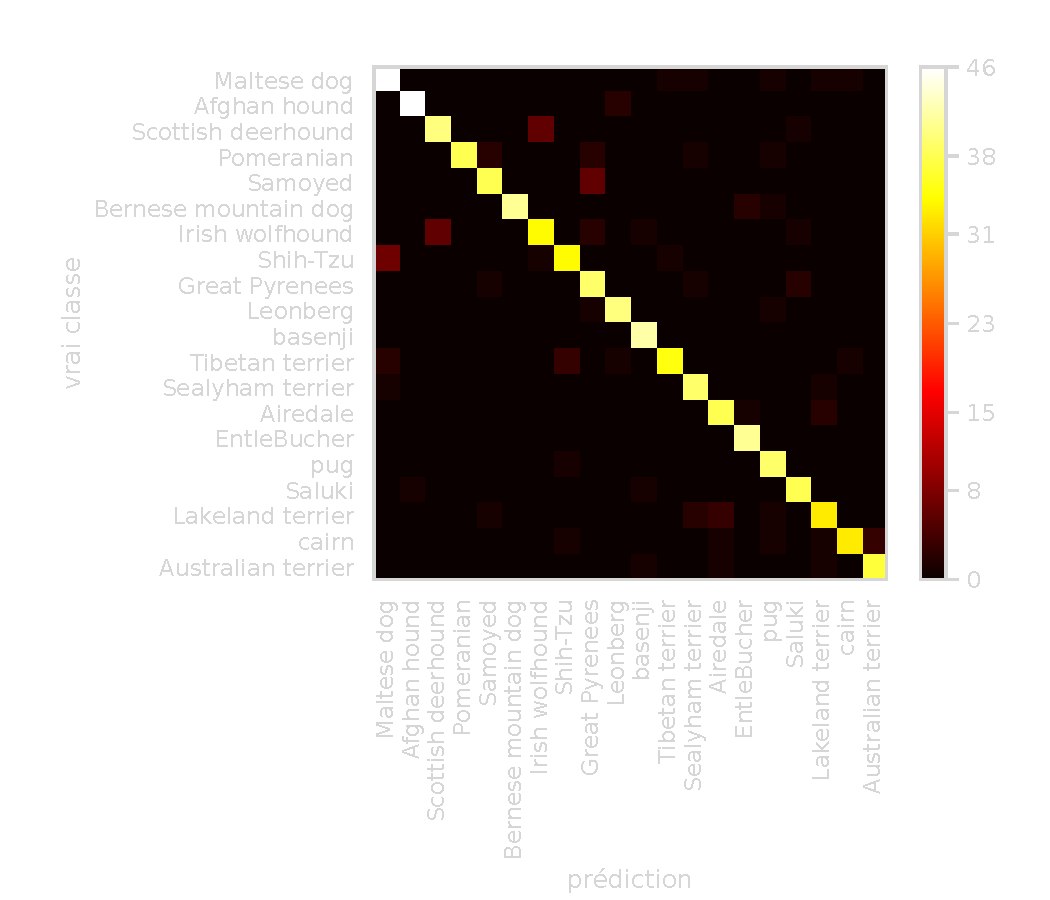
\includegraphics[width=80mm]{results/confusion.pdf}
			} ;

			\begin{scope}[xshift=-30mm, yshift=18mm]
				\node<3->{
					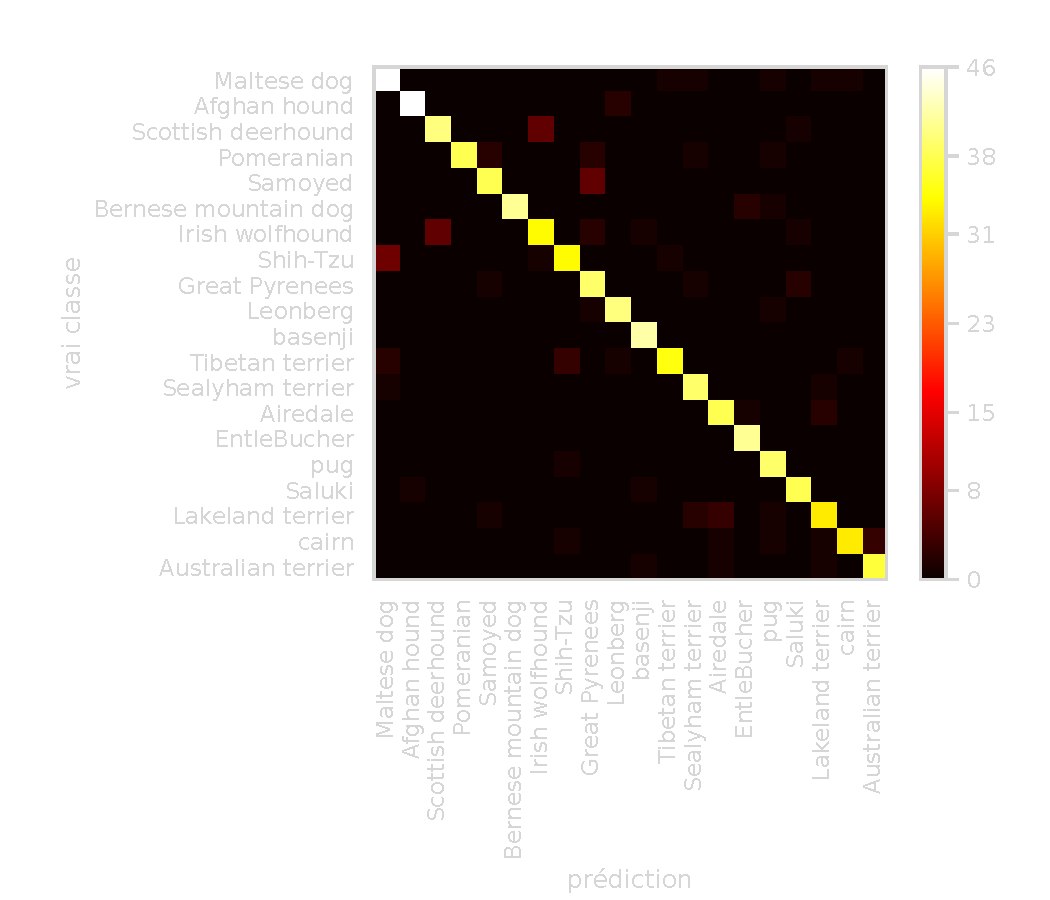
\includegraphics[width=40mm]{results/confusion.pdf}
				} ;
			\end{scope}


			\begin{scope}[xshift=20mm, yshift=20mm]
				\node<4-> {
					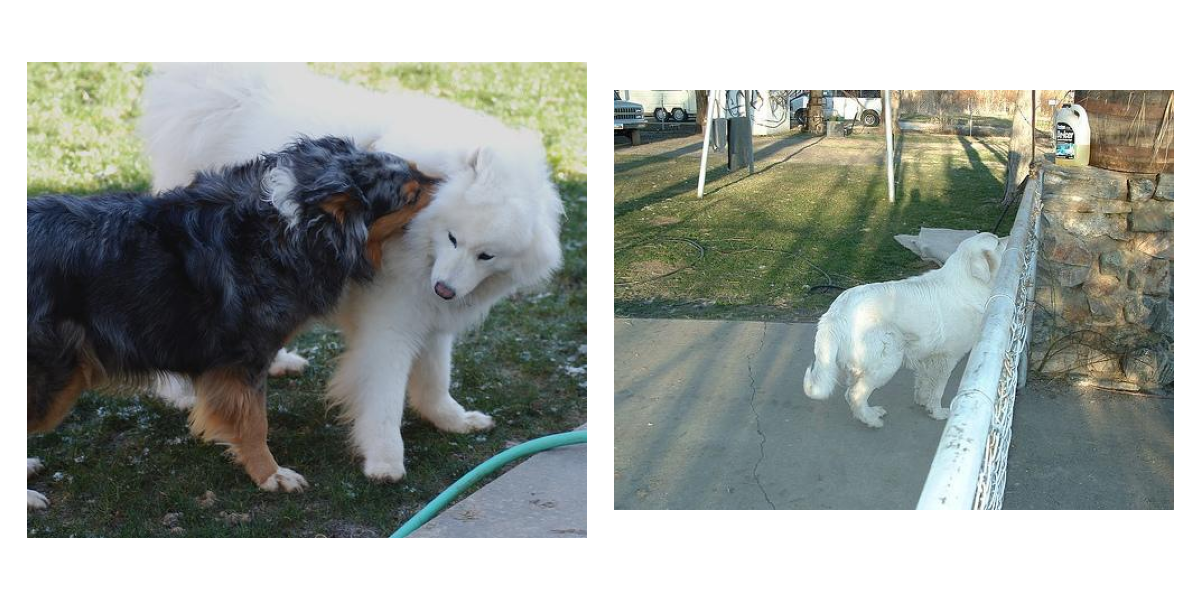
\includegraphics[width=60mm]{results/example_close_classes2.png}
				} ;
			\end{scope}
			\begin{scope}[xshift=0mm, yshift=-10mm]
				\node<5-> {
					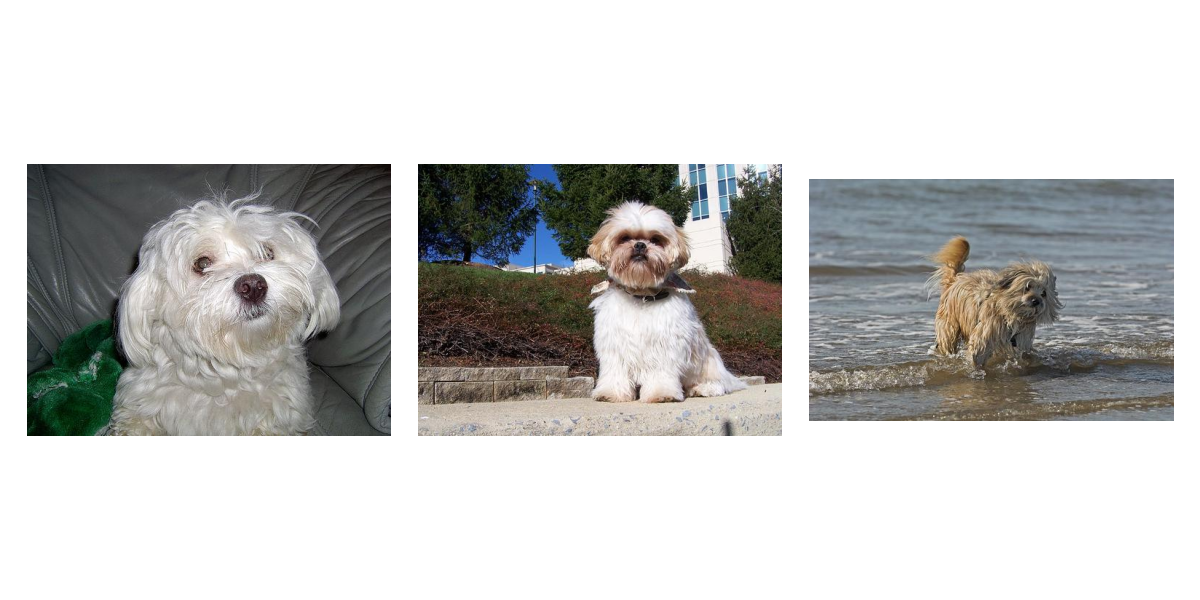
\includegraphics[width=70mm]{results/example_close_classes1.png}
				} ;
			\end{scope}

			\node<6-> at (0, -25mm) {On obersve de \alert{fortes ressemblances} entre \alert{certaines races}} ;
			\node<7-> at (0, -35mm) {Surtout avec les possibilités \alert{poils longs} / \alert{courts}} ;
		\end{scope}

	\end{tikzpicture}
	\vfill
\end{frame}

\section{CONCLUSIONS}
\begin{frame}[t, label=CCL]
	\vspace{0mm}
	\centering
	\vfill
	\begin{tikzpicture}
		\linespread{1}% <--- locally defined vertical line spacing in nodes
		\drawBorder
		\nodePageNumber

		\onlystyle<2->{shd1}{myShaded}
		\onlystyle<3->{shd2}{myShaded}
		\onlystyle<4->{shd3}{myShaded}
		% \onlystyle<5->{shd4}{myShaded}
		% \onlystyle<6->{shd5}{myShaded}
		% \onlystyle<7->{shd6}{myShaded}
		\begin{scope}[xshift=\midX, yshift=-3mm]
			\node[shd1, text centered, text width=90mm] at (0,80mm) {Entrainer un \alert{réseau profond} nécessite \alert{beaucoup de données}} ;
			\node<2->[shd2, text centered, text width=90mm] at (0,60mm) {Les \alert{modules}, les fonctions d'\alert{activation} et l'\alert{architecture} sont \alert{à optimiser}} ;
			\node<3->[shd3, text centered, text width=90mm] at (0,40mm) {L'utilisation de \alert{modèles pré-entrainés} \alert{accélère} l'apprentissage et \alert{réduit} la \alert{quantité de données nécessaire}} ;
			\node<4>[text centered, text width=90mm] at (0,20mm) {Il reste des \alert{erreurs} de \alert{prédiction} liées à de \alert{fortes similiratités} entre certaines \alert{races}} ;
		\end{scope}

	\end{tikzpicture}
	\vfill
\end{frame}

\begin{frame}[t, label=Perspectives]
	\vspace{0mm}
	\centering
	\vfill
	\begin{tikzpicture}
		\linespread{1}% <--- locally defined vertical line spacing in nodes
		\drawBorder
		\nodePageNumber

		\onlystyle<2->{shd1}{myShaded}
		\onlystyle<3->{shd2}{myShaded}
		\onlystyle<4->{shd3}{myShaded}
		% \onlystyle<5->{shd4}{myShaded}
		% \onlystyle<6->{shd5}{myShaded}
		% \onlystyle<7->{shd6}{myShaded}
		
		\begin{scope}[xshift=\midX, yshift=-3mm]
			\node[shd1, text centered, text width=90mm] at (0,80mm) {\alert{Amélioration} du \alert{code d'entrainement} (réduction des calculs de loss/metric entrainement)} ;
			\node<2->[shd2, text centered, text width=90mm] at (0,60mm) {Entrainement sur \alert{plus de classes}} ;
			\node<3->[shd3, text centered, text width=90mm] at (0,40mm) {Récupération de \alert{plus de données}} ;
			\node<4>[text centered, text width=90mm] at (0,20mm) {Utilisation de \alert{visual transformers}} ;
		\end{scope}
	\end{tikzpicture}
	\vfill
\end{frame}

\begin{frame}[t, label=Merci]
	\vspace{0mm}
	\centering
	\vfill
	
\begin{tikzpicture}
		\linespread{1}% <--- locally defined vertical line spacing in nodes
		\drawBorder

		\node at (0.5\textwidth,\midY) {\huge \alert{Merci} pour votre \alert{attention}.} ;

	\end{tikzpicture}
	\vfill
\end{frame}

\end{document}
